% !TEX TS-program = pdflatex
% !TEX encoding = UTF-8 Unicode

% This is a simple template for a LaTeX document using the "article" class.
% See "book", "report", "letter" for other types of document.

\documentclass[11pt]{article} % use larger type; default would be 10pt

%\usepackage[utf8]{inputenc} % set input encoding (not needed with XeLaTeX)


%%% Examples of Article customizations
% These packages are optional, depending whether you want the features they provide.
% See the LaTeX Companion or other references for full information.

%%% PAGE DIMENSIONS
\usepackage{geometry} % to change the page dimensions
\geometry{a4paper} % or letterpaper (US) or a5paper or....
\geometry{margin=1in} % for example, change the margins to 2 inches all round
% \geometry{landscape} % set up the page for landscape
%   read geometry.pdf for detailed page layout information

\usepackage{graphicx} 
% \usepackage[parfill]{parskip} % Activate to begin paragraphs with an empty line rather than an indent

%%% PACKAGES
%\usepackage{booktabs} % for much better looking tables
\usepackage{array} % for better arrays (eg matrices) in maths
%\usepackage{paralist} % very flexible & customisable lists (eg. enumerate/itemize, etc.)
\usepackage{verbatim} % adds environment for commenting out blocks of text & for better verbatim
%\usepackage{subfig} % make it possible to include more than one captioned figure/table in a single float
% These packages are all incorporated in the memoir class to one degree or another...

%%% HEADERS & FOOTERS
\usepackage{fancyhdr} % This should be set AFTER setting up the page geometry
\pagestyle{fancy} % options: empty , plain , fancy
\renewcommand{\headrulewidth}{0pt} % customise the layout...
\lhead{}\chead{}\rhead{}
\lfoot{}\cfoot{\thepage}\rfoot{}

%%% SECTION TITLE APPEARANCE
%\usepackage{sectsty}
%\allsectionsfont{\sffamily\mdseries\upshape} % (See the fntguide.pdf for font help)
% (This matches ConTeXt defaults)

%%% ToC (table of contents) APPEARANCE
%\usepackage[nottoc,notlof,notlot]{tocbibind} % Put the bibliography in the ToC
%\usepackage[titles,subfigure]{tocloft} % Alter the style of the Table of Contents
%\renewcommand{\cftsecfont}{\rmfamily\mdseries\upshape}
%\renewcommand{\cftsecpagefont}{\rmfamily\mdseries\upshape} % No bold!

%\usepackage[T1]{fontenc}
\usepackage[latin9]{inputenc}
%\usepackage[active]{srcltx}
\usepackage{setspace}
\doublespacing
\usepackage[english]{babel}
\begin{document}

\title{Connectivity Analysis of Metagenomic Data}
\author{ACH, JP, RCK, RM, JJ, JMT, CTB}
\maketitle

\section{Introduction}
Given the rapid decrease in the costs of sequencing, we can now achieve the sequencing depth necessary to study even the most complex environments \cite{Hess:2011p686,Qin:2010p189}.  The main bottleneck for such metagenomic studies is the lack of effective strategies to annotate and predict gene functions from the enormous sequencing datasets that are now being generated \cite{Hoff:2009p913,Kunin:2008p16,Noguchi:2006p968,Zhang:2012p959}.  In general, de novo metagenomic assembly has been used as a solution, mainly because it significantly reduces the data size by collapsing numerous short reads into fewer contigs and provides longer sequences containing multiple genes and operons \cite{Miller:2010p226,Pop:2009p798}.  Furthermore, because it does not rely on the availability of reference genomes, it also produces novel contigs allowing for comparisons of these sequences within and between metagenomes \cite{Li:2009p707,Schloss:2008p2} or annotations of unknown genomes \cite{Hess:2011p686}.  The success of de novo metagenomic assembly, however, relies on the ability to store information about the connectivity of sequencing reads within an assembly graph and thus is limited by both the amount of sequencing and the availability of computational memory. 

To deal with these limitations, new metagenome-specific de novo assemblers use various approaches to break apart components of the assembly graph  \cite{Peng:2011p898} (cite metaVelvet).  These assemblers take advantage of the fact that environmental populations contain multiple genomes which have been sampled at varying depths reflecting their natural abundance.  Read coverage (the extent to which sequencing reads contribute to assembled contigs) and/or graph connectivity are used to break apart and simplify metagenomic assembly graphs. 

The ability to resolve connected components of an assembly graph depends on accurately distinguishing variable-coverage genome sequences from sequencing errors and bias.  The presence of sequencing biases and errors are known to be present in Illumina sequences \cite{Harismendy:2009p228,Hoffmann:2009p1027,Nakamura:2011p741} but very little is known about their effects on assembly graph properties and the resulting assemblies.  With large amounts of sequencing (a requirement for complex metagenomes), increases in the number of real biological sequences are accompanied by increases in sequencing errors and biases.  In this study, we analyzed the ability to resolve connected components of several metagenomic assembly graphs.  In doing so, we identified highly-connecting sequences in several metagenomes which we demonstrate originate from sequencing artifacts.  We evaluated the effects of removing these sequences on metagenomic assembly and discuss how this approach ultimately enables the assembly of large, complex metagenomes.  

\section{Results}

\subsection{Connectivity analysis of metagenome datasets}

\subsubsection{Presence of a single, highly-connected lump in all datasets}
We selected datasets from three diverse, medium to high complexity metagenomes from the human gut \cite{Qin:2010p189}, cow rumen \cite{Hess:2011p686}, and agricultural soil (unpublished). For comparison, we also included one simulated metagenome (error-free) of a high complexity, high coverage (\textasciitilde{}10x) microbial community \cite{Pignatelli:2011p742}. To study the effects of increased sequencing, we also included two additional subsets of the agricultural soil metagenome containing 50 million and 100 million reads each.

The connectivity of reads within the assembly graph of each dataset was evaluated within a de Bruijn graph representation (see Methods).  Reads contributing to disconnected portions of the assembly graph were separated.  In each dataset, we identified a dominant, highly-connected set of sequencing reads which we referred to as a "lump" (Figure 1, Table 1).  In the simulated dataset, this lump consisted of 5\% of the reaads.  In the studied metagenomes, the lump ranged from 7\% (in the smallest soil metagenome) to 76\% (in the human gut metagenome).  In a smaller subset of the human gut metagenome (50 million reads), the relative size of the lump was similar and comprised over 75\% of the sequencing reads (data not shown).  For the three soil datasets, the increase in the size of the lump was not proportional to increases in the amount of sequencing (Figure 1, Table 1).  As the number of reads increased by 2-fold and 5-fold, the size of the lump increased by 5-fold and 14-fold, respectively.  

\begin{figure}
\center{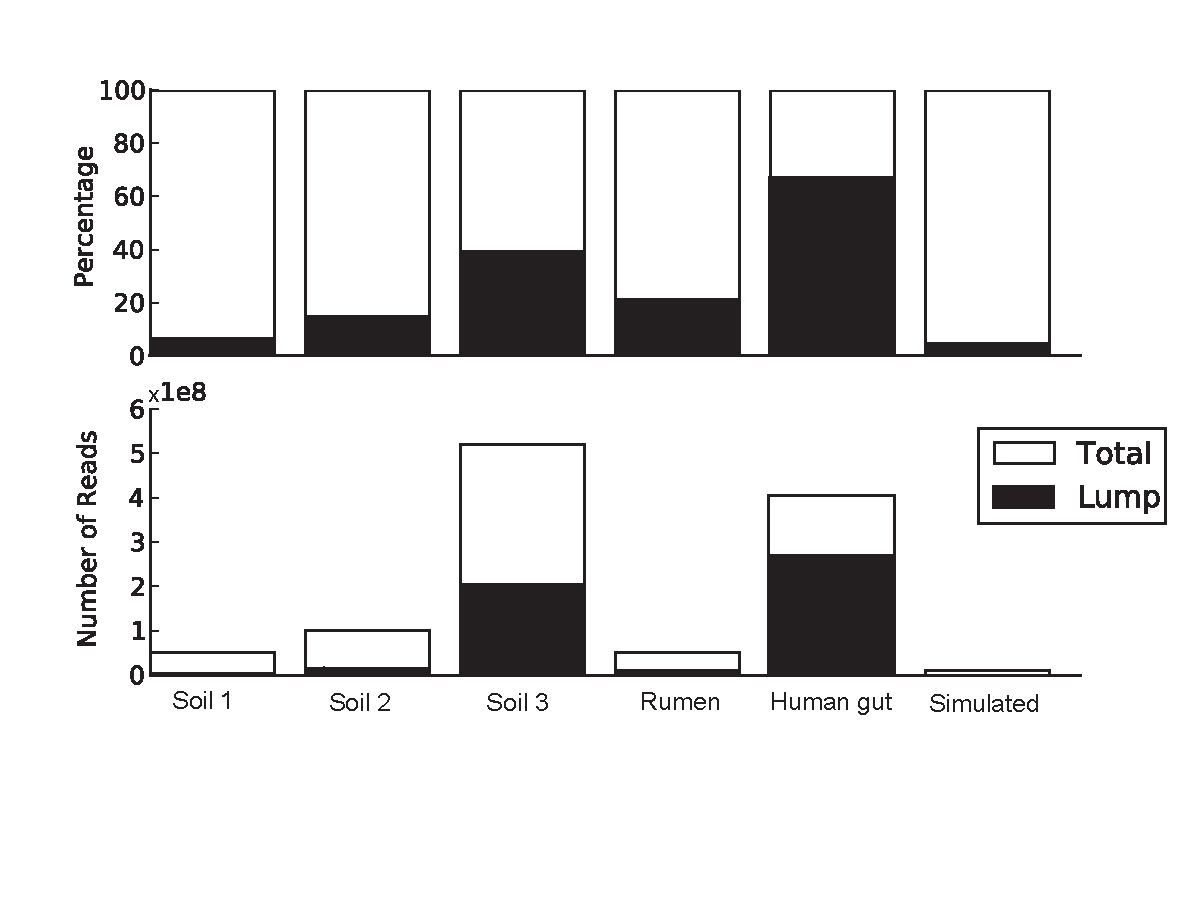
\includegraphics[width=5in]{./figures/lump_sizes.png}}
\caption{Within each metagenome, a dominant set of connected reads was identified which we refer as a lump.}
\end{figure}



@This supra-linear increase of lump size relative to the increase of number of reads suggests that the connectivity of reads within a lump increases more rapidly than the contents of the lump.  
@Note that filtering out highly abundant k-mers effects - CTB, need to analyze

\subsubsection{Characterizing assembly graphs in metagenomic and simulated lumps}

To assess the degree of connectivity of sequences within the lump, we measured the local graph density of reads within the de Bruijn assembly graph.  The local graph density is defined here as the number of k-mers, or sequences of length k, found within a distance of N divided by N.  In the case of a linear sequence, the local graph density would be 2; additional branches or repeats would increase this value.  For the mixture of 112 bacterial genomes used for the simulated dataset, fewer than 2\% of the nodes within the assembly graph had an average graph density greater than 20.   For the lump in the simulated reads, 17\% of the nodes had an average graph density greater than 20.  Within the metagenomic datasets, average graph density greater than 20 ranged from 21 to 50\%.  

@Will insert table here

We next determined the extent to which graph density varied by position along sequenced reads by measuring the average local graph density within ten steps of every k-mer by position in a read (Figure 2).  For the simulated dataset, the average local density was stable for all positions along reads.  In contrast, metagenome datasets had increased average local graph densities which varied depending on read position.  

\begin{figure}
\center{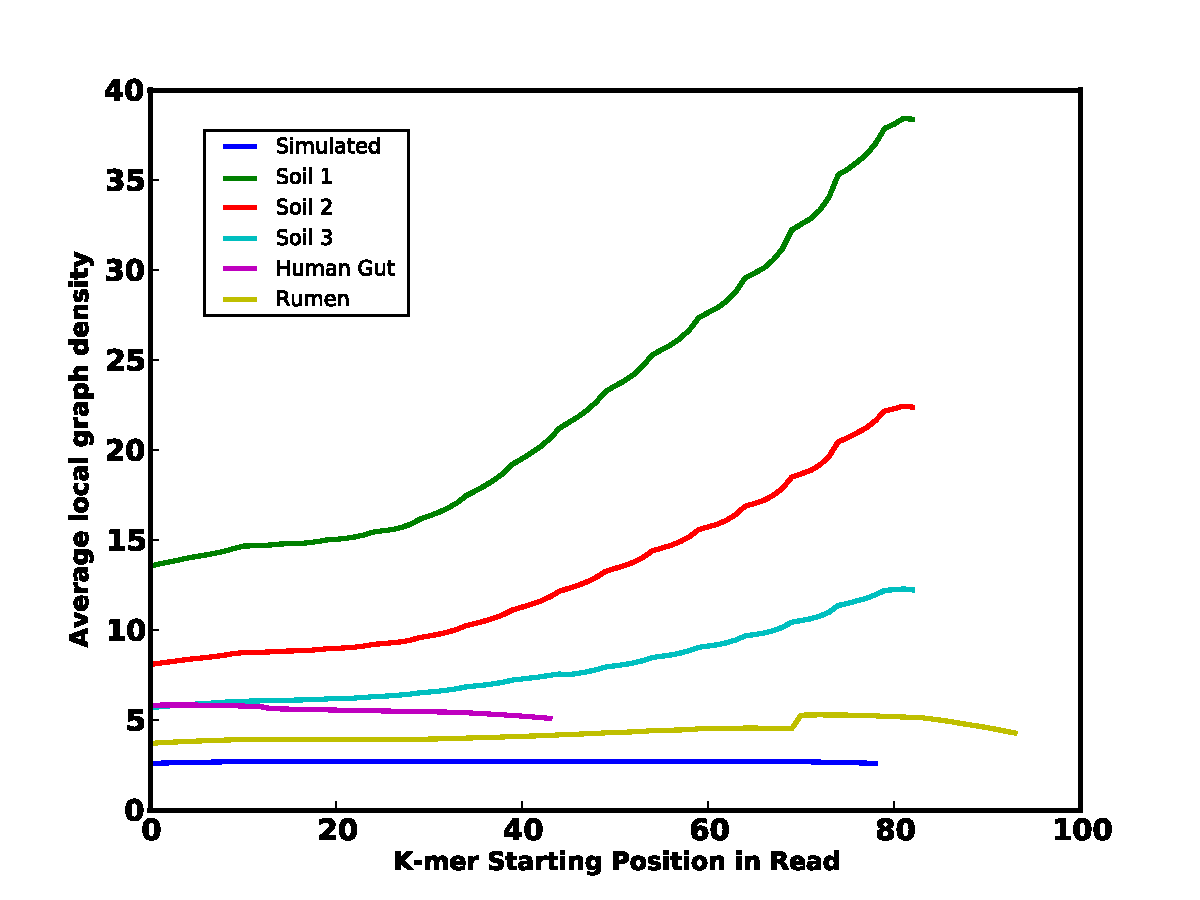
\includegraphics[width=5in]{./figures/density_pos.png}}
\caption{Graph density indicates the degree of connectivity between sequences.  In contrast to the simulated lump, graph density varied by position in sequenced reads in metagenomic lumps.}
\end{figure}

\subsection{Identification of highly-connecting k-mers and their effects on assembly}

\subsubsection{Characteristics of highly-connecting sequences in simulated and metagenomic lump reads}

We identified sequences within each lump which were causes of high-connectivity using a systematic assembly graph traveral algorithm (see Methods).  In general, 6 to 8\% of the unique k-mers within metagenomic lumps and 3\% of unique k-mers within the simulated lump were found to be knot-causing sequences.  An exception was the smallest soil (50 million reads) lump which contained than less than 1\% of the unique, highly-connective k-mers.

@Insert table of stoptag \% here

Subsequently, we compared the lumps in all datasets by assessing the extent to which these k-mers were found at specific positions along a sequencing read.  The presence of highly-connecting k-mers in simulated reads did not exhibit any bias with regard to position within the read.  However, in all metagenomic datasets, highly-connecting k-mers were more prevalent at position-specific locations along the read (Figure X).  

\begin{figure}
\center{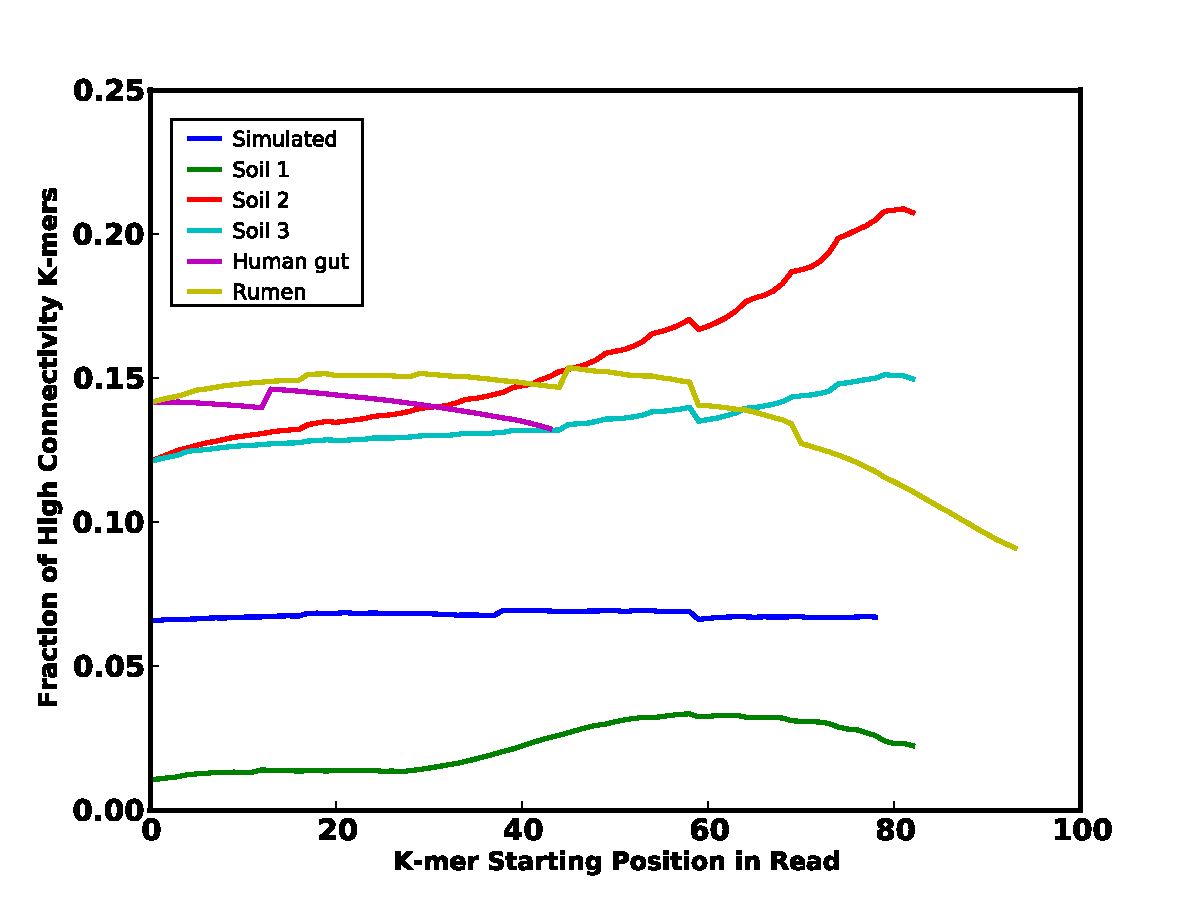
\includegraphics[width=5in]{./figures/position_read.png}}
\caption{Highly-connecting sequences (k-mers) were present with position-specific bias within sequencing reads in metagenomic data.}
\end{figure}


\subsubsection{Characteristics of highly-connecting sequences in simulated and metagenomic lump assemblies}

We evaluted the incorporation of the highly-connecting k-mers into the final assembly of the lumps.  For all lumps, we found that the proportion of unique knot-causing k-mers in assembled contigs (longer than 500 bp) were significantly less than that of originating sequencing reads.  In the simulated lump, there was an 8-fold enrichment of these sequences in the reads compared to the final assembly.  In metagenomic lumps, highly-connecting k-mers averaged ~5x (this number will likely change with minimus) enrichment in sequencing reads over assembled contigs (Table X).  We also examined the position of these highly-connecting k-mers within assembled contigs.  For all datasets, we found that these sequences were being disproportionately placed on the ends of contigs (Figure X).  

@This table will be changed with minimus results - need to do minimus for metagenomic datasets.

\begin{figure}
\center{\includegraphics[width=5in]{./figures/knot_enrichment_in_reads.pdf}}
\caption{Highly-connecting k-mers were more highly enriched in sequencing reads compared to assembled contigs, suggesting poor incorporation by assembly.}
\end{figure}

@Effects of removing these highly connecting lumps on the the lump, discuss breaking up lump by removing these guys...

\begin{figure}
\center{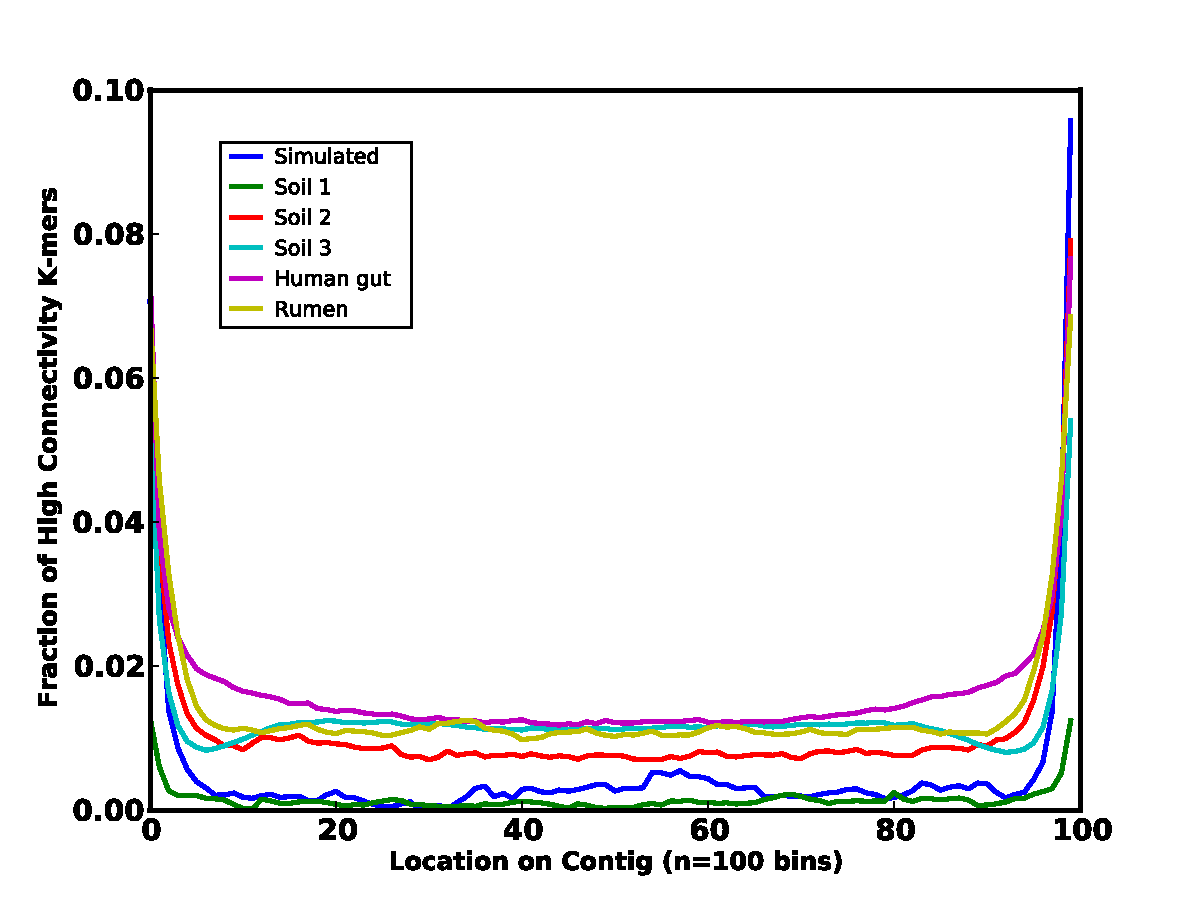
\includegraphics[width=5in]{./figures/pos-spec-bias-contigs.png}}
\caption{When incorporated into an assembly, highly-connecting sequences (k-mers) were disproportionately present at the ends of contigs.}
\end{figure}

\subsubsection{Effects of removing highly-connecting k-mers on the simulated lump assembly}
We removed the above identified knot-causing k-mers from reads to assess their effects on downstream assembly.  In the error-free simulated dataset, we assembled both the unfiltered and knot-filtered lump.  Overall, the number of contigs (longer than 500 bp) and length of assembly was improved by filtering knot-causing k-mers.  The unfiltered assembly contained 1,844 contigs (maximum size = 3,787 bp) with 1,365,436 bp, while the knot-filtered assembly contained 2,301 contigs (maximum size = 5,826 bp) with 1,733,645 bp.

From these assemblies, we predicted open reading frames (ORFs) from assembled contigs with lengths greater than 500 bp (see Methods).  The unfiltered and knot-filtered assembly contained 2,401 and 3,049 ORFs, respectively.  To evaluate the accuracy of assembly, we compared these ORFs to the 112 genomes from which the simulated dataset orginated.  In the unfiltered lump assembly, 2,395 (99.8\%) of ORFs matched the reference genomes.  The knot-filtered lump assembly contained more assembled ORFs, 3,037 (99.6\%) which matched the reference genomes.  We found that the unfiltered and knot-filtered assemblies shared 2,018 ORFs.  A total of 383 and 1,031 ORFs were unique to the unfiltered and knot-filtered assemblies, respectively.   
Furthermore, comparing the constitutive k-mers making up the unfiltered and knot-filtered assemblies (see Methods), we estimate that these assemblies are approximately 31\% different.  

We compared the 2,018 ORFs which were identified in both the unfiltered and knot-filtered assemblies by aligning these sequences to the best match protein from the reference genomes.  Overall, we found that there was a slight improvement in the alignment length of knot-filtered compared to unfiltered ORFs (Figure X).

@@need to fix axes

\begin{figure}
\center{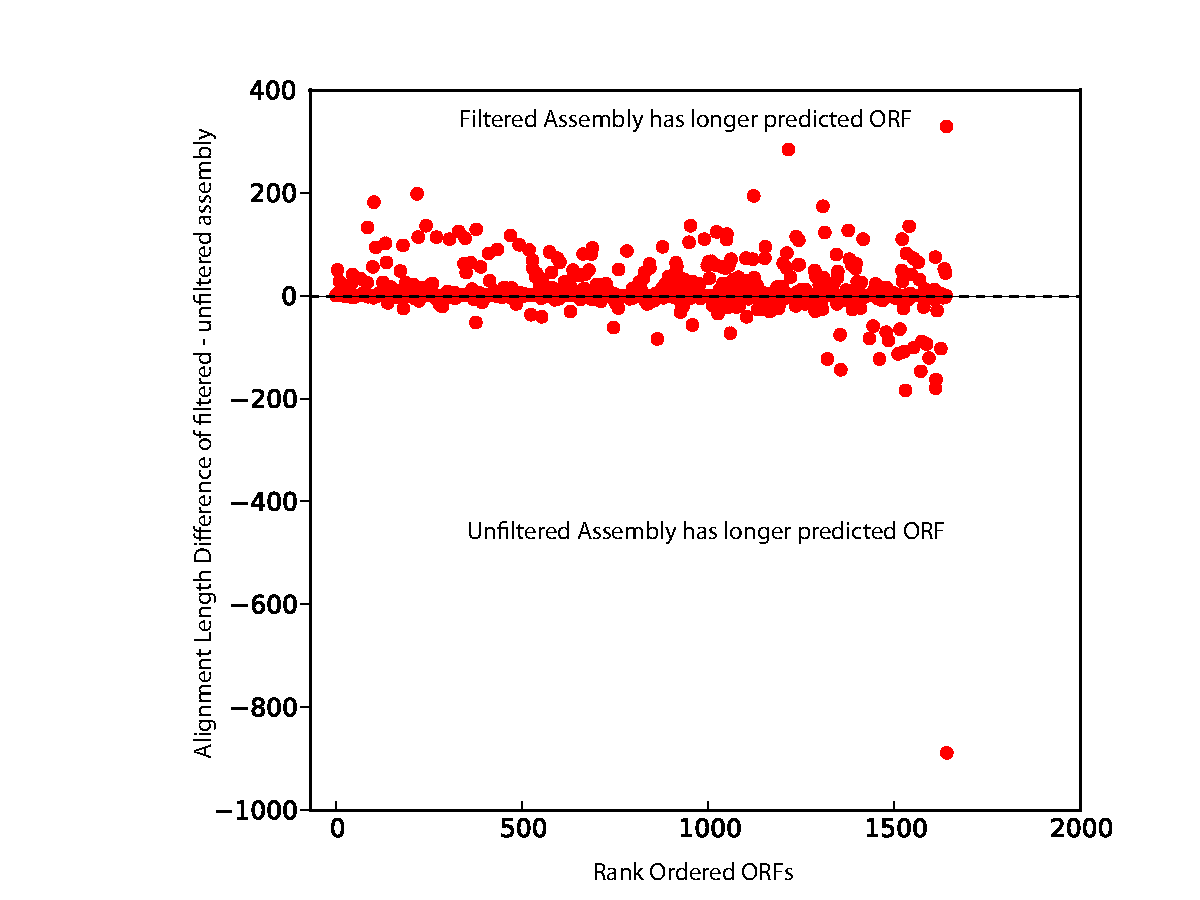
\includegraphics[width=5in]{./figures/orf_lengths.png}}
\caption{Alignment lengths of knot-filtered compared to unfiltered ORFs to reference genome proteins.  The difference of the alignment length of filtered and unfiltered ORFs is shown for increasing predicted ORF lengths (ranked by filtered assembly), average=3.7 bp, stdev=35.8 bp, median=0 bp.}
\end{figure}


@@are the unique orfs shorter? - small signal, not sure if good enough if strong enough to include here

\section{Discussion}

\subsection{Characteristics of the lump did not appear to be biological in origin.}

We were able to separate several metagenomic assembly graphs into millions of disconnected assembly subgraphs representing sequences originating from different genomes.  The largest of these subgraphs, called the lump, contained a disproportionate number of reads relative to other subgraphs.  Initially, we considered that this lump consisted mainly of connecting sequences which were conserved across multiple genomes (i.e. 16S rRNA, ITS regions).  However, efforts to remove conserved genes from datasets did not significantly break apart the lump (data not shown).  The large size of the lump within metagenomic data compared to that of a simulated metagenomes (i.e., 75\% of reads in the human gut metagenome vs. 5\% in simulated) also suggested some connectivity within this lump was not biological.  Furthermore, we observed that with increasing sequencing (in the soil metagenomes), there was a supra-linear increase in the size of the lump and thus graph connectivity (Figure X). These results combined indicated that possible spurrious connectivity was present in metagenomic lumps, and we proceeded to further analyze the connectivity these sequences.

\subsection{Position-specific biases indicate that sequencing artifacts are present in the lump.}
We first assessed the degree of connectivity within the lump by measuring the local graph density of metagenomic lumps.  For a mixture of genomes, the local graph density was measured to be low, less than 2\% of nodes with graph density greater than 20.  For the lump of connected reads of a simulated Illumina sequencing dataset of these genomes, the graph density (as expected for a connected lump) is larger with 17\% of nodes having a graph density greater than 20.  For the metagenomic lumps studied, the degree of connectivity is consistently larger than the simulated data, on average 35\% of metagenomic nodes had a graph density greater than 20.   In addition to increased connectivity, we observed varying local graph densities with respect to the position within a read in all metagenomes (Figure X).  This position-specific bias, not observed in the simulated dataset, clearly suggested spurrious connectivity among metagenomic sequences.

To further explore the sources of this spurrious connectivity, we identified the highly-connecting sequences within each lump which were likely causes of the lump itself.  Similarly to the observed position-specific bias of local graph density along the read, highly-connecting sequences also had a biased presence in locations of sequencing reads (Figure X).  Given that shotgun sequencing is randomly generated, these observed biases strongly suggests that these highly-connecting sequences are not biological and are the result of sequencing artifacts.  

\subsection{Comparing position-specific trends in various metagenomes indicates preferential attachment.}
For each metagenome, similar position-specific trends were observed for both graph density and the proportion of highly-connecting sequences (Figures X and X).  Among the metagenomes studied, the position-specific biases (toward the 3' end of the read) was most pronounced in the two largest soil metagenomes (100 million and 500 million reads).  Overall, for the soil metagenomes, the size of the lump and associated position-specific trends, increased at a greater rate than the amount of sequencing.  We suspect that this is the result of an effect referred to as "preferential attachment" \cite{Barabasi:1999p1083}. In this case, highly connecting "X" sequences in a lump recruit a number of connecting "Y" reads into the lump.  As more sequences are added, these "Y" reads, which do not necessarily have to be highly-connective, recruit more "Z" reads into the lump resulting in increasingly larger lump size.  For soil metagenomes (where sequencing coverage is relatively low and diversity is high), more sequencing may cause preferential attachment of "X", "Y", and "Z" reads resulting in increasingly larger lump sizes.  For metagenomes of less complexity, like that of the human gut and cow rumen, the number of the "Y" and "Z" reads which are lump-associated but not highly-connective would increase (because of greater sequencing coverage) at a greater rate than than "X" reads.   This would effectively introduce a greater proportion of sequences in the lump which would not be identified as highly-connective and result in an overall decrease in the total fraction of these sequences.   This reasoning is supported by the observation that the total number of identified unique highly-connecting sequences (6-8/%) was consistent between all metagenomes, with the exception of the smallest soil.  Given the same proportion of highly-connecting sequences are present in all metagenomes, differences in trends likely originate from characteristics of the metagenomes themselves (i.e. sequencing coverage).  We speculate that the smallest soil metagenome is a special case because of its low coverage and high diversity.

@?
@ still need to add coverage data in

\subsection{Removing highly-connecting sequences improves assembly overall.}
Although some of the highly-connecting sequences in metagenomic lumps are sequencing artifacts (given their position-specific bias), we know that not all of these sequences are non-biological because we have identified 3\% of unique k-mers in the error-free simluated dataset as highly-connective.  However, regardless of the origin of these sequences, we were interested in their incorporation into resulting assemblies.

For all datasets studied, we observed that these sequences were under-represented in the final assembly compared to their presence in original sequencing reads.  Moreover, when these sequences were incorporated into assembly, they tended to begin or end contigs.  These results suggest that, overall, the assemblers are challenged by characteristics of these sequences.  We thus speculated that the removal of these sequences would have little effect on the final assembly. 

The simulated dataset was an ideal case study because it contained no sequencing errors or biases and could be validated by the original reference genomes.  We compared the assembly of the simulated dataset before and after filtering out highly-connected sequences to evaluate the biological effects of these sequences on assembly.  In general, the unfiltered and filtered assemblies were quite different based on constituent k-mer composition (31% different) and unique ORFs (34\% ORFs unique to only the filtered assembly).  The removal of highly-connecting sequences, however, improved assembly overall.  Comparing the resulting assemblies, the filtered assembly contained 29\% more contigs and 51\% longer assembly length (for contigs greater than 500 bp).  Additionally, the filtered assembly predicted 27\% more ORFs which had matches to reference genomes.  Among the shared 2,018 ORFs between assemblies, those originating from the filtered assembly had longer alignment lengths to proteins predicted from the originating reference genomes (Figure X).  These results indicate that removing highly-connecting sequences, even if originating from real biological connectivity, can improve the overall assembly.  

@Next add in rumen validation where we have the genomes from the assembly generated, and stats for assembly for the rest of the metagenomes, need to run metasim...


\section{Conclusion}
Removing these lumps is computationally very useful, enabling MetaIDBA as well as scaling approaches

\bibliography{artifacts-paper-bib}
\bibliographystyle{plain}


\end{document}